%\documentclass[handout]{beamer}
\documentclass[ignorenonframetext]{beamer}
\usepackage{textpos}
\usepackage{graphicx}
\usepackage{pgf}
\usepackage{caption}
\usepackage{listings}
\usepackage{multimedia}
\usepackage{gensymb}
\usepackage{amsmath, mathrsfs}

% \captionsetup[figure]{labelformat=empty}% redefines the caption setup of the figures environment in the beamer class.

\usetheme{Boadilla}
\usefonttheme{serif}
% \mode<presentation>
% {
%  \usefonttheme{serif}
% % \useoutertheme{sidebar}
% %   \logo{\includegraphics[height=1cm]{elec_logo.pdf}}
% }

\title[TART]{The Transient Array Radio Telescope (TART): An overview}
\author[Molteno]{Tim Molteno}

\institute[Otago]
{
  Electronics Research Foundation \\
  \& \\
  Department of Physics,
  University of Otago \\
  \vspace{1cm}
  \large{Dunedin, New Zealand.}\\
  \vspace{2cm}
  \includegraphics[width=0.6\linewidth]{../tart_overview/fig/elec_header_font.pdf}
}

\logo{\pgfputat{\pgfxy(-0.72,7.7)}{\pgfbox[center,base]{\includegraphics[width=1cm]{../tart_overview/fig/elec_logo.pdf}}}}

\date[CbU June 2025] % (optional, should be abbreviation of conference name)
{}

\begin{document}

% Abstract: In this talk I'll give an overview of Africa's newest radio telescope, the TART, recently installed in Mauritius in a joint effort between SARAO, the University of Otago (NZ). I'll talk about TARTs origins, it's design and open-source philosophy as well as the upcoming project to install TART telescopes in the SKA African partner nations. I'll also include some details about improvements that will appear in TART-3, the next version of TART!

\begin{frame}
  \titlepage
\end{frame}
 
\begin{frame}
\vspace{1cm}

  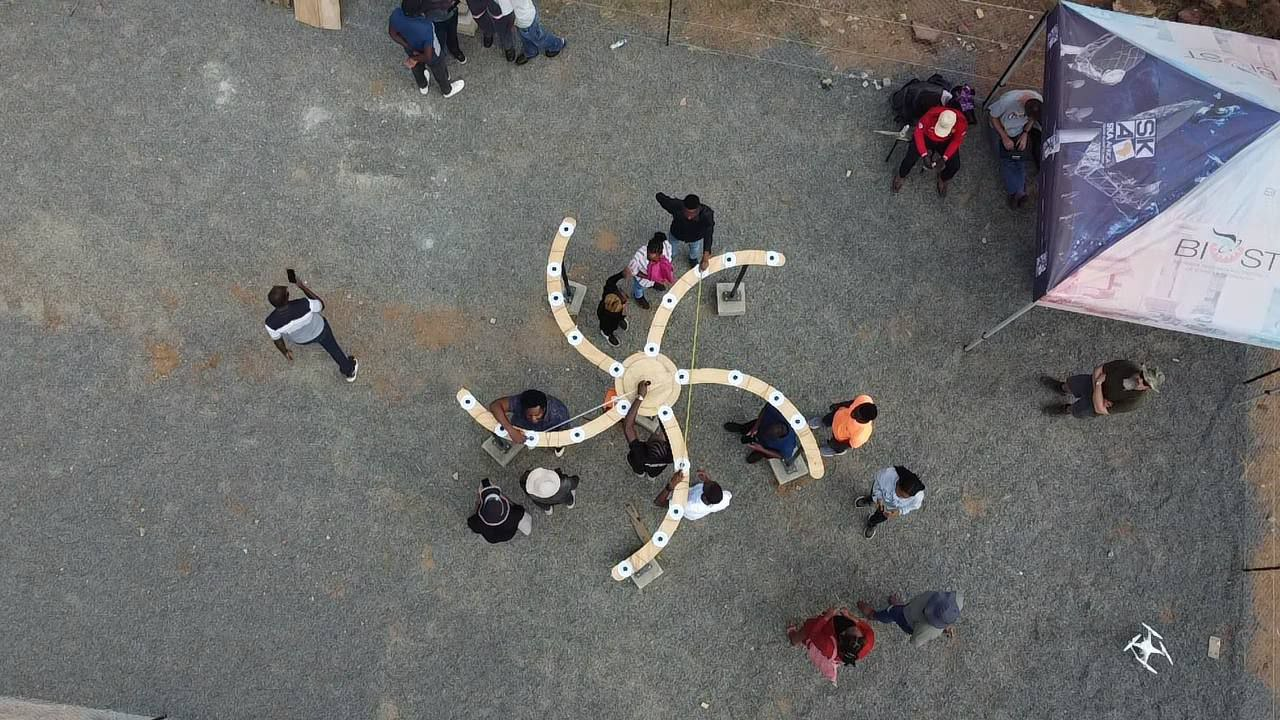
\includegraphics[width=\linewidth]{fig/biust_from_above.jpg}\\
  \centering{BIUST TART final calibration. Yesterday!}
\end{frame}

% \begin{frame}{Abstract}
%  I will introduce the Transient Array Radio Telescope. Developed here in the Department of Physics at Otago University, this is the worlds smallest (and cheapest) aperture synthesis radio telescope -- that is a telescope that creates images of the radio sky. It is now being used by astronomers working on the Square Kilometer Array, the worlds largest radio telescope -- as an instrument that can be used to both develop new algorithms for radio astronomy and also to teach students about how radio telescopes work. I will describe the instrument and how it works, as well as giving an overview of the upcoming projects involving this telescope in Africa.
% \end{frame}

\begin{frame}
  \tableofcontents
  % You might wish to add the option [pausesections]
\end{frame}

\section{Goals of this workshop}

% \begin{frame}{Goals of the workshop}
% \begin{}
%
% \end{frame}
% \section{Origins of TART}

\begin{frame}{TART: Single-Dish Engineering Prototype}
   \includegraphics[width=\linewidth]{fig/albatross_frame.png}
\end{frame}

\begin{frame}{TART: Evaluation}
   \includegraphics[width=\linewidth]{fig/project_map_14.png}
\end{frame}


%  \begin{columns}
%   \begin{column}{0.5\linewidth}
%   \begin{center}
%     \includegraphics[height=0.4\textheight]{fig/antenna.jpg}
%   \end{center}
%   \end{column}
%   \begin{column}{0.5\linewidth}
%    \includegraphics[width=\textwidth]{fig/antenna.jpg}
%   \end{column}
%  \end{columns}
% 

% \section{Aperture synthesis Radio Telescopes}

% 
% \begin{center}
%   \includegraphics[width=0.45\linewidth]{fig/RadioNightSky_med.jpg}
%   \includegraphics[width=0.45\linewidth]{fig/green_bank.jpg}
% \end{center}
% \end{frame}

% \begin{frame}{Aperture synthesis Radio Telescopes}
% \begin{center}
%   \includegraphics[width=\linewidth]{fig/vla_large.jpg}
% \end{center}
% \end{frame}


\begin{frame}{MeerKAT: Africa is a world-leader in radio astronomy}
\begin{center}
  \includegraphics[width=\linewidth]{fig/2018-MeerKAT-5-1030x355.jpg}
\end{center}
\begin{itemize}
 \item 13.5 meter antennas. 143 $m^2$
 \item 64 of them!
 \item Frequency Range: 900 MHz - 1670 MHz
 \item SKA pathfinder
\end{itemize}

\end{frame}


% \begin{frame}{MeerKAT: The Centre of our Galaxy}
%  \begin{center}
%   \includegraphics[width=\linewidth]{fig/MeerKAT_GalacticCentre_image.jpeg}
%  \end{center}
% 
% \end{frame}


\begin{frame}{MeerKAT: It's very precious}
MeerKAT \& ASKAP \& VLA \& GMRS are amazing radio telescopes
\begin{itemize}
\item Beautiful engineering
\item Total cost: billions
\item Running cost: millions
\item A long queue of eager astronomers...
\end{itemize}

\begin{block}{STEM research}
 Testing new ideas is almost impossible.
\end{block}

\includegraphics[width=0.32\linewidth]{fig/ska-logo-color.pdf}
\includegraphics[width=0.32\linewidth]{fig/NRF_SARAO_sm1.png}
\includegraphics[width=0.32\linewidth]{fig/ska-partners.png}
\end{frame}

\section{TART: A telescope designed for research}

\frame{\tableofcontents[currentsection]}

% 
% \begin{frame}
%   \includegraphics[width=\linewidth]{fig/rhodes_opening.jpg}
% \end{frame}
% 
% \begin{frame}
%   \includegraphics[width=\linewidth]{fig/rhodes_photo_array.jpg}
%   \includegraphics[height=0.4\textheight]{fig/rhodes_photo_elec.jpg}
% \end{frame}



\begin{frame}{TART-2: Overview}
   \includegraphics[width=\textwidth]{fig/drone_view_rhodes.jpg}
   \centering{all-sky  $\cdot$ 24 antennas $\cdot$ real-time $\cdot$ open-source $\cdot$ imaging interferometer } 
\end{frame}




\mode<all>
{
\usebackgroundtemplate{\includegraphics[height=\paperheight]{fig/tart_udm_array.jpg}}
\begin{frame}[plain]
\end{frame}
}
\mode<all>{\usebackgroundtemplate{}}

\mode<all>
{
\usebackgroundtemplate{\includegraphics[height=\paperheight]{fig/tart2_wiring_mess.jpg}}
\begin{frame}[plain]
\end{frame}
}
\mode<all>{\usebackgroundtemplate{}}


\subsection*{Open Source}


% \begin{frame}{TART-2: Installation in South Africa}
% \begin{center}
%   \includegraphics[width=0.9\linewidth]{fig/rhodes_photo_array.jpg}
% \end{center}
% \begin{itemize}
%  \item 0.025 meter antennas. 0.0005 $m^2$.
%  \item Frequency Range: 1575.42 MHz ($\pm 4$)
%  \item Dunedin, NZ, Rhodes \& Stellenbosch South Africa.
% \end{itemize}
% \end{frame}
% 
% \begin{frame}
% \vspace{1cm}
%   \includegraphics[width=\linewidth]{fig/rhodes_news_sa.jpg}
% \end{frame}

\begin{frame}{TART is open-source}
  \centering\url{https://github.com/tart-telescope}
 \begin{columns}
  \begin{column}{0.4\linewidth}
    \begin{itemize}
      \item Designed for Research
      \item Github: Hardware
      \item Github: Software
      \item Github: Documentation
    \end{itemize}
    
    Contributors:
    \begin{itemize}
      \item Dunedin, NZ
      \item Rhodes, ZA
      \item Stellenbosch, ZA
      \item SARAO, ZA
      \item AlphaWave, ZA
      \item Volunteers from industry
    \end{itemize}
  \end{column}
  \begin{column}{0.6\linewidth}
    \includegraphics[width=\linewidth]{fig/screenshot_github.png}
  \end{column}
  \end{columns}
\end{frame}

 
\begin{frame}{TART-2 components}
  \includegraphics[width=\linewidth]{fig/tart_overview.pdf}
\end{frame}



\begin{frame}{GPS receiver chips}
 \begin{columns}
  \begin{column}{0.5\linewidth}
    \includegraphics[width=\linewidth]{fig/max_2769.jpg}
  \end{column}
  \begin{column}{0.4\linewidth}
  GPS silicon devices in TART:
\begin{itemize}
 \item Operates at 1575 MHz (19cm)
 \item Low-cost, widely available
 \item 2.5 MHz bandwidth
 \item 16 millions bits per second
\end{itemize}
  \end{column}
  \end{columns}
\end{frame}



\begin{frame}{TART-3 Electronics}
 \includegraphics[width=\textwidth]{fig/tart3_boxed.jpg}
\end{frame}

\begin{frame}{TART-3 Features}
 \begin{columns}
  \begin{column}{0.4\linewidth}
    \begin{itemize}
    \item 32-Antennas (276 $\rightarrow$ 496 Visibilities)
    \item New Correlator will support up to 64 Antennas!
    \item 2-bit data!
    \item New radios: $10 \times$ bandwidth
    \end{itemize}
  \end{column}
  \begin{column}{0.6\linewidth}
    \includegraphics[width=\linewidth]{fig/tart3.jpg}
  \end{column}
\end{columns}
\pause
    \begin{block}{Sensitivity}
Sensitivity increase of ~$20 \times$
    \end{block}
    \begin{block}{Reliability}
Simplified wiring. Much easier installation. Easier to maintain.
    \end{block}
\end{frame}



\begin{frame}{Upgraded Radios, late 2025}
  \begin{columns}
  \begin{column}{0.4\linewidth}
    \includegraphics[width=\linewidth]{fig/max2771.png}
  \end{column}
  \begin{column}{0.6\linewidth}
  New Radio Front End.
\begin{itemize}
 \item 10x bandwidth (26 MHz)
 \item Zero IF operation
 \item 1160-1290 MHz and 1525-1610 MHz bands
 \item New radio module, will plug into existing TARTs.
\end{itemize}

  \end{column}
  \end{columns}
\end{frame}

\begin{frame}{New Array Layouts}
\centering
 \includegraphics[width=0.33\linewidth]{fig/top_view.jpg}
 \includegraphics[width=0.54\linewidth]{fig/drone_view_rhodes.jpg}
 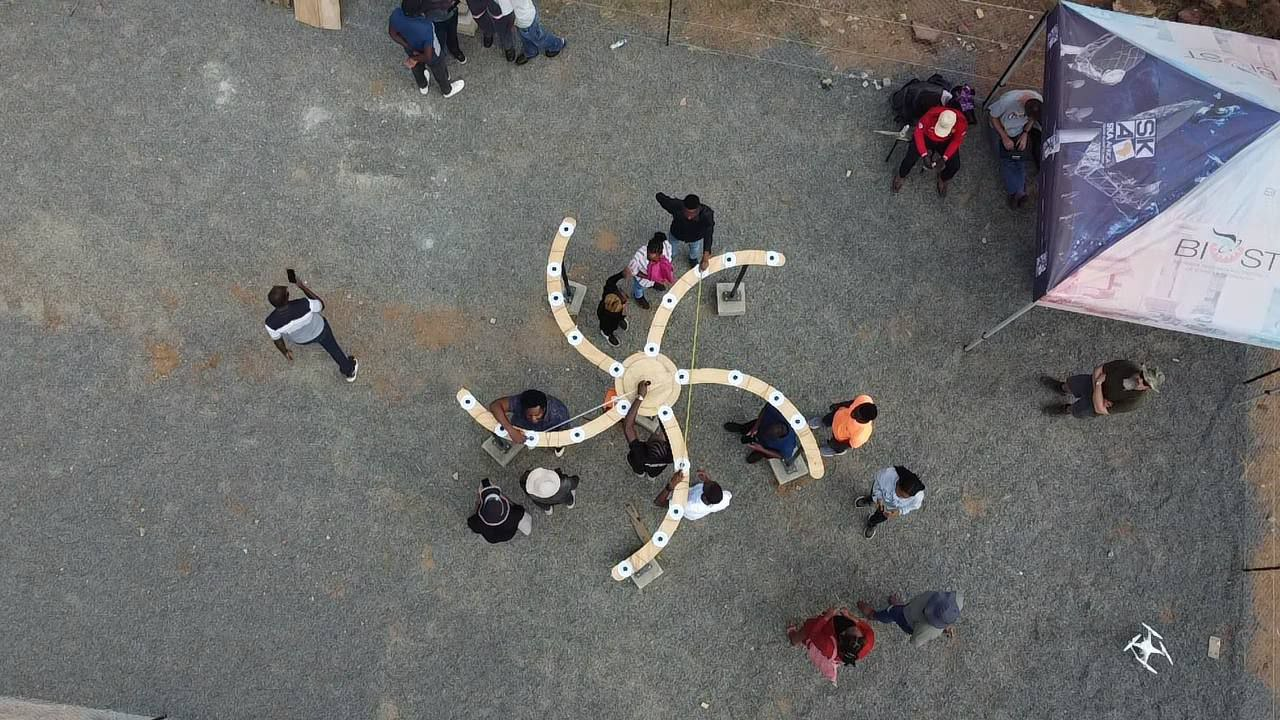
\includegraphics[width=0.6\linewidth]{fig/biust_from_above.jpg}
\end{frame}

\section{Calibration Imaging \& Data}

\frame{\tableofcontents[currentsection]}


\begin{frame}{The Calibration Sources}
 \begin{columns}
  \begin{column}{0.5\linewidth}
   \includegraphics[height=0.9\textheight]{fig/QZS-1.jpg}
  \end{column}
  \begin{column}{0.5\linewidth}
  \begin{itemize}
   \item Position known to millimeters
   \item $>20000$ km away (point sources)
   \item Signal is `noise-like'
  \end{itemize}
   \includegraphics[width=\textwidth]{fig/qzss_ground_track.jpg}
   {\tiny Image: JAXA}
  \end{column}
 \end{columns}
\end{frame}

\begin{frame}
 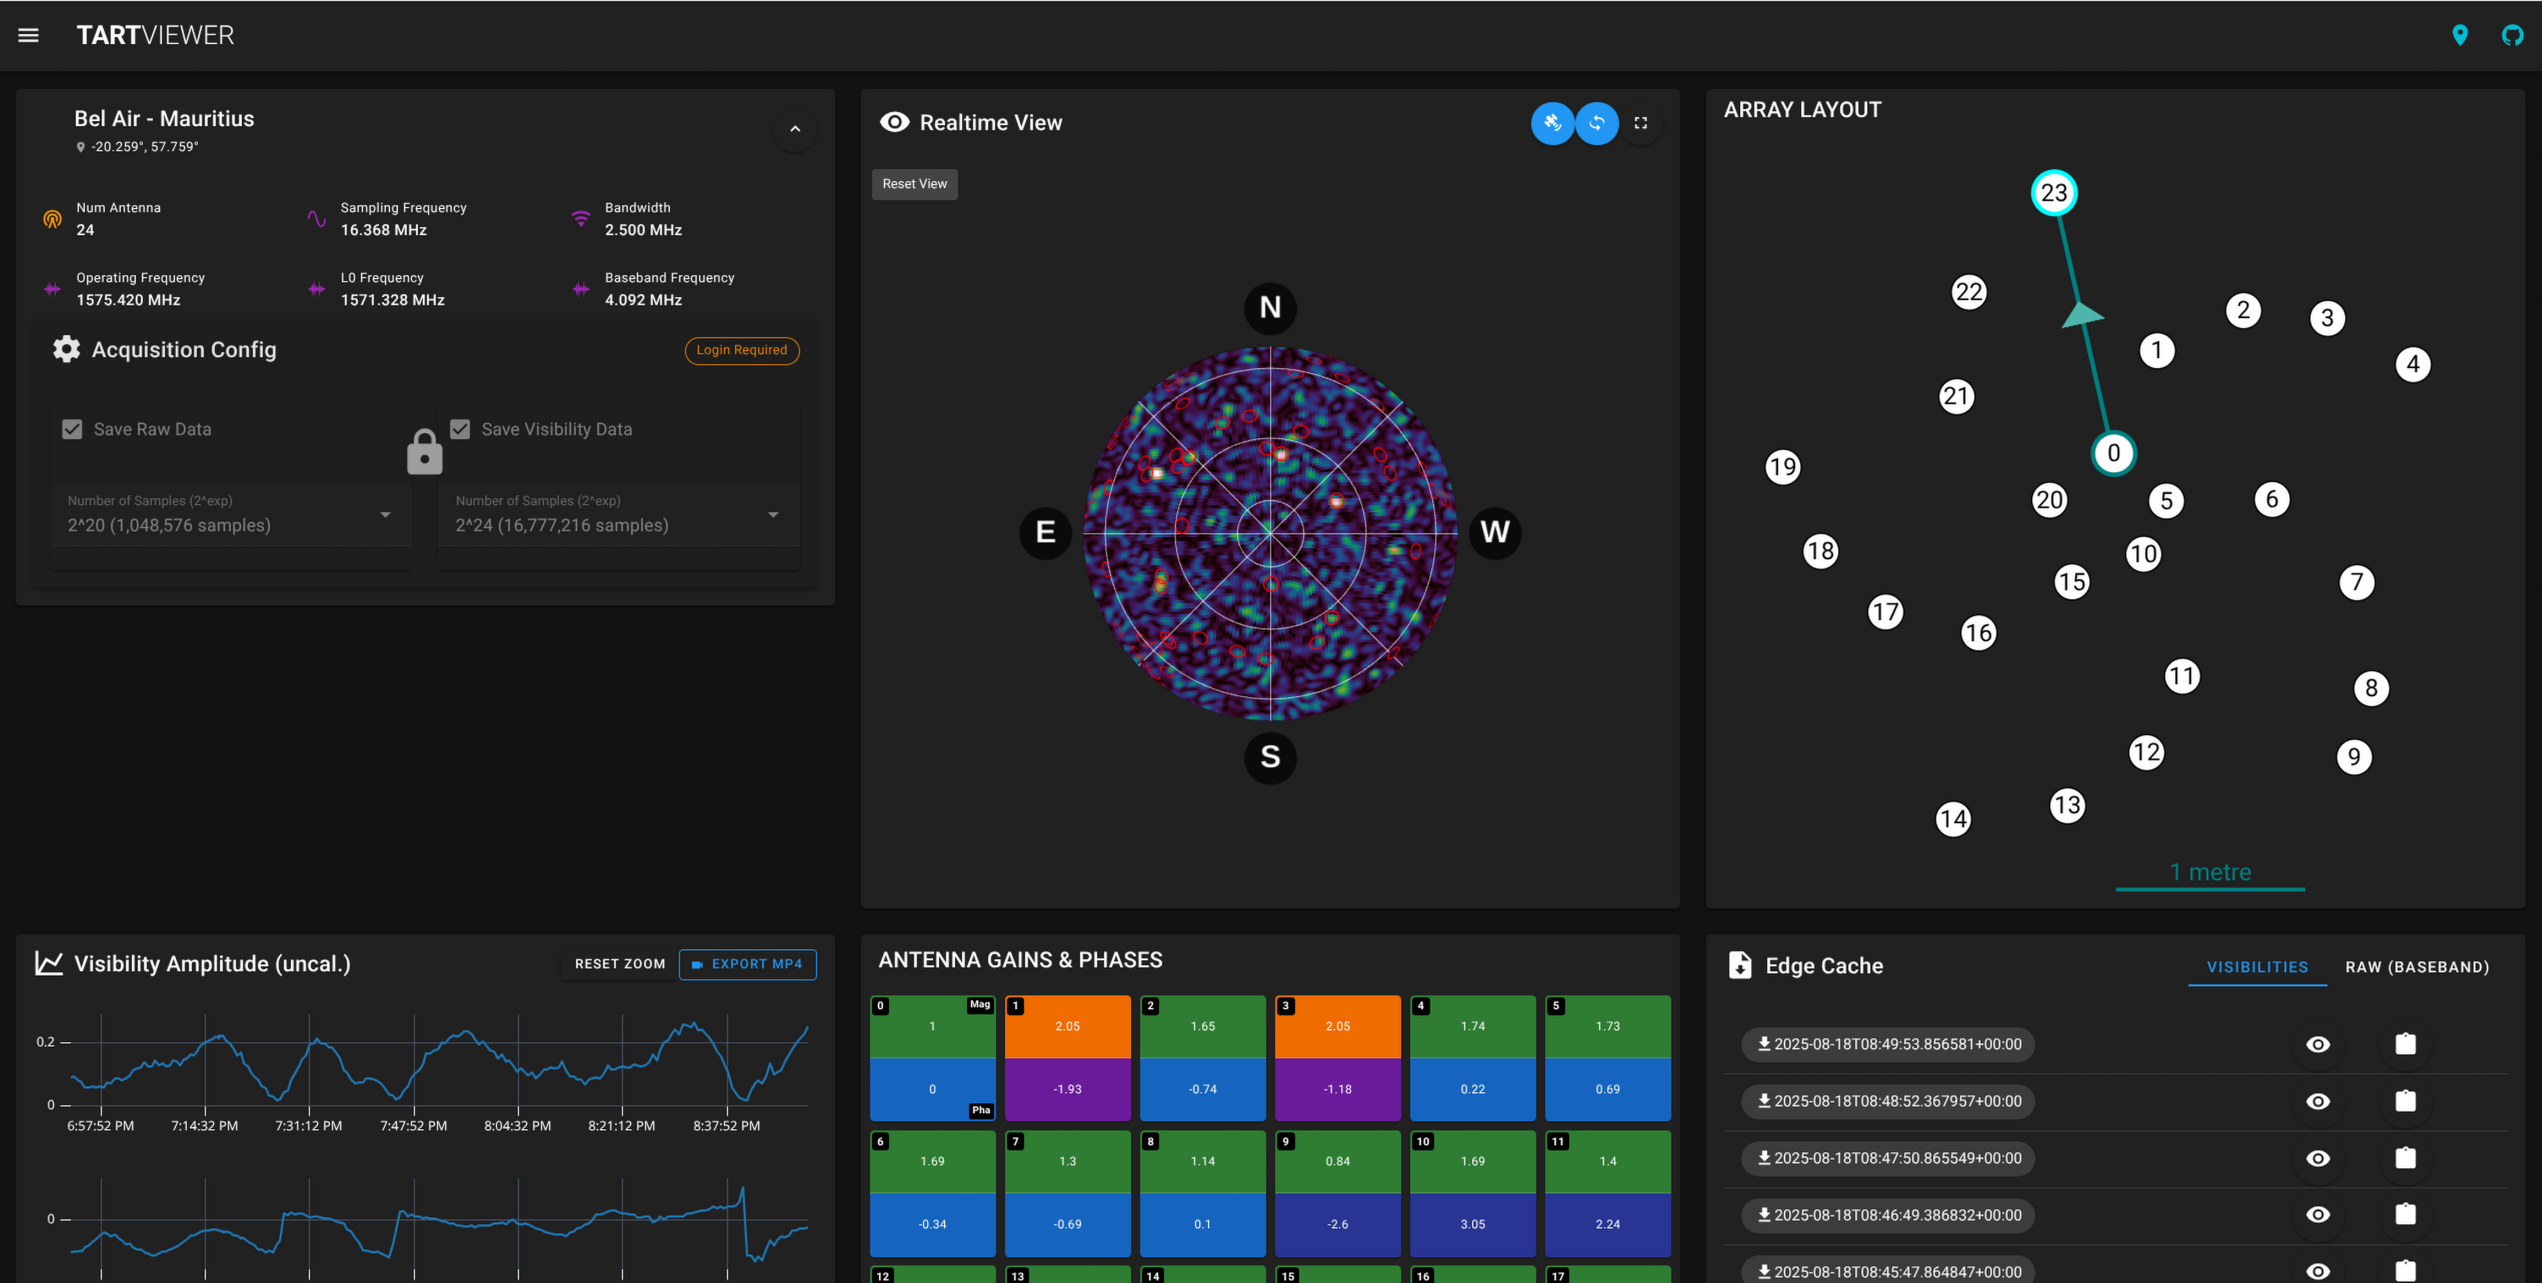
\includegraphics[width=\linewidth]{fig/browser_view.png}
\end{frame}

% \begin{frame}[containsverbatim]
% \frametitle{TART API: Access data from anywhere}
% TART data and control are done throught a web-based API.
%
% \centering{\url{https://api.elec.ac.nz/tart/tart3-test/}}
%
% \begin{lstlisting}[language=Python, frame=single, basicstyle=\footnotesize]
%  import requests
%
%  api_endpoint = "https://api.elec.ac.nz/tart/tart3-test/api/"
%  r = requests.get(api_endpoint + "/v1/imaging/vis")
%  print(r.json())
% \end{lstlisting}
%
% \end{frame}

% \begin{frame}{Synthesis Imaging}
% Measure complex visibility $V_{ij}$ by correlating signals from antenna $i$ and $j$.
% \[ V_{ij} = \frac{1}{T} \int_0^T E_i(t) E_j^{\star}(t) dt \]
% \begin{columns}
%  \begin{column}{0.55\linewidth}
% \begin{enumerate}
%  \item 276 Pairs of antennas
%  \item 16.368 MHz sampling rate per antenna
%  \item Real-time correlation in FPGA
%  \item 4.5 Giga MAC per second
%  \item T $\sim$ 1 second
% \end{enumerate}
%  \end{column}
%  \begin{column}{0.45\linewidth}
%  \includegraphics[width=\linewidth]{fig/papilio_pro.jpg}
%  \end{column}
% \end{columns}
% 
% \end{frame}
% 
% \begin{frame}{Synthesis Continued...}
% Fourier transform relationship between radio sky brightness $I(l,m)$ and
% visibility $V(u,v)$,
% \[
%   V(u,v) = \int I(l,m) e^{2\pi j(lu  + mv)} dl dm
% \]
% Obtain $I(l,m)$ through inverse Fourier transform of $V(u,v)$, 
% \[
%  I(l,m) = \mathscr{F}^{-1}\{V(u,v)\}
% \]
% where $V(u,v)$ is the visibility function sampled in the $uv$-plane at the locations of each antenna $(u_{ij},v_{ij})$ pair. 
% \end{frame}
% 

% \section{Expected \& Unexpected Results}

\begin{frame}{Tart Imaging Results}
\begin{center}
\includegraphics[width=0.6\linewidth]{fig/tart_snapshot.pdf}\\
 \url{https://tart.elec.ac.nz/old/strange_flyby.webm}
 \end{center}
\end{frame}

\begin{frame}{UFO}
\begin{center}
\includegraphics[width=0.8\linewidth]{fig/elaz.jpg}\\
 Consistent with something in low-earth orbit.
 \end{center}
\end{frame}

% 
% 
% \begin{frame}{The Dirty Image}
% For the TART telescope there are 24 antennas, 
% and 522 antenna pairs
% \begin{columns}
%  \begin{column}{0.5\textwidth}
%  \begin{figure}
% \includegraphics[width=\linewidth]{../../papers/2019_iceaa/uv_plane_init.pdf}
% \caption{U-V antenna pairs}
%  \end{figure}
%  \end{column}
%  \begin{column}{0.5\textwidth}
%  \begin{figure}
%  \includegraphics[width=\linewidth]{fig/beam_2017_10_21_19_38_39_UTC.png}
% % \includegraphics[width=\linewidth]{/home/tim/github/projects/max/phd/talk/nzip/pdf/dirty_beam_power_init.pdf}  
% \caption{Inverse Fourier Transform}
%  \end{figure}
%  \end{column}
% \end{columns}
% 
% \end{frame}
% % 
% % 
% % \begin{frame}{Swithing it on: Uncalibrated Image}
% % \begin{figure}
% % \includegraphics[height=0.9\textheight]{../../papers/2019_iceaa/uncalibrated_image.png} 
% % \end{figure}
% % \end{frame}
% % 
% % 
% % % \begin{frame}{CLEAN: H\"ogbom 1974}
% % % \begin{columns}
% % %  \begin{column}{0.5\linewidth}
% % % %  \includegraphics[width=\linewidth]{2017_10_21_19_38_39_UTC_uvfits_difmap.png}
% % %   \end{column}
% % %  \begin{column}{0.5\linewidth}
% % %   Image is the sum of point sources and a residual
% % %   \begin{eqnarray*}
% % %  I(l,m) & = & A_0 \delta(l_0, m_0) + I_0(l,m) \\
% % %  I_0(l,m)  & = & A_1 \delta(l_1, m_1) + I_1(l,m) \\
% % % 	   & = & \ldots
% % %   \end{eqnarray*}
% % %  \end{column}
% % % \end{columns}
% % % \end{frame}
% % 
% % 
% 
% 
% \begin{frame}{Calibrated Clean Image}
% \begin{center}
% \includegraphics[height=0.9\textheight]{{../../papers/2019_iceaa/tart_clean.png}}
% \end{center}
% \end{frame}


\section{The TART Workshops}

\frame{\tableofcontents[currentsection]}

\begin{frame}{Workshops: Building the TART Community}
 \begin{columns}
  \begin{column}{0.4\linewidth}
\includegraphics[width=\linewidth]{fig/Africa.pdf}
  \end{column}
  \begin{column}{0.6\linewidth}
  \begin{itemize}
   \item Week-long workshops
   \item Mornings: Lectures on radio astronomy
   \item Afternoons: Building a TART
   \item Collaboration between members
   \item Including schools (2025 \& 2026)
  \end{itemize}
\end{column}
 \end{columns} 
 \centering
   \includegraphics[width=0.71\linewidth]{fig/workshop-partners.png}
\end{frame}



\begin{frame}{What the future holds}
 \begin{columns}
  \begin{column}{0.6\linewidth}
    \begin{itemize}
    \item TART 4.0?
    \item Transient event detection
    \item More workshops! Bangaladesh, Morrocco, Malta, Berkeley
    \item Automatic tracking of space Debris
    \item New Array Designs
    \item New imaging algorithms (Gridless, Direct from Data)
    \end{itemize}
  \end{column}
  \begin{column}{0.4\linewidth}
    \includegraphics[width=\linewidth]{fig/tart3.jpg}
  \end{column}
\end{columns}
    \pause
    \begin{block}{}
     \begin{center} Questions? \end{center}
    \end{block}

\end{frame}



\end{document}
